\documentclass[oneside]{ctexart}
\usepackage[a4paper,left=2.5cm,right=2.5cm,top=2.8cm,bottom=2.5cm]{geometry}
\usepackage{amsmath,amssymb,mathtools,bm}
\usepackage{booktabs}
\usepackage{graphicx}
\usepackage{float}
\usepackage{xcolor}
\usepackage{listings}
\usepackage[colorlinks=true,linkcolor=blue,urlcolor=blue,citecolor=blue]{hyperref}

\lstset{
    language=Python,
    basicstyle=\small\ttfamily,
    keywordstyle=\color{blue!60!black},
    commentstyle=\color{green!40!black},
    stringstyle=\color{red!50!black},
    numbers=left,
    numberstyle=\tiny,
    stepnumber=1,
    numbersep=8pt,
    breaklines=true,
    showstringspaces=false,
    frame=single,
    tabsize=4
}

\DeclareMathOperator{\Var}{Var}
\DeclareMathOperator{\Cov}{Cov}
\DeclareMathOperator{\Pois}{Pois}
\DeclareMathOperator{\diag}{diag}
\newcommand{\dd}{\,\mathrm{d}}

\begin{document}

\section{第 2 题:ordinary renewal process 的更新函数统计量}

设普通更新过程的更新间隔为
\[
    X_1,X_2,\ldots,
\]
并假设它们独立同分布,分布函数为 $F$.记
\[
    S_k=X_1+\cdots+X_k,
    \qquad S_0=0,
\]
则时刻 $t$ 前的更新次数为
\[
    N(t)=\max\{k:S_k\leq t\}.
\]
这里 $N(t)$ 就是 renewal counting function.因为
\[
    \{N(t)=k\}=\{S_k\leq t<S_{k+1}\},
\]
所以它的分布可以写成
\begin{equation}
    \mathbb P(N(t)=k)=F^{*k}(t)-F^{*(k+1)}(t),\qquad k=0,1,2,\ldots,
\end{equation}
其中 $F^{*k}$ 表示 $F$ 的 $k$ 重卷积,并约定 $F^{*0}(t)=1$.

因此,$N(t)$ 的 $n$ 阶原点矩为
\begin{equation}
    \mathbb E[N(t)^n]
    =\sum_{k=0}^{\infty} k^n\bigl(F^{*k}(t)-F^{*(k+1)}(t)\bigr).
\end{equation}
这个公式是最直接的精确表达式.

也可以用下降阶乘矩写得更紧凑.记
\[
    (x)_r=x(x-1)\cdots(x-r+1),
\]
则
\begin{equation}
    \mathbb E[(N(t))_r]
    =r!\sum_{k=r}^{\infty}\binom{k-1}{r-1}F^{*k}(t),
    \qquad r=1,2,\ldots .
\end{equation}
这是因为当 $N(t)=m$ 时,右端内部的组合数满足
\[
    \sum_{k=r}^{m}\binom{k-1}{r-1}=\binom{m}{r}.
\]
再利用第二类 Stirling 数 $\left\{\begin{matrix} n\\ r\end{matrix}\right\}$,有
\begin{equation}
    N(t)^n=\sum_{r=1}^{n}
    \left\{\begin{matrix} n\\ r\end{matrix}\right\}(N(t))_r .
\end{equation}
于是得到
\begin{equation}
    \boxed{
    \mathbb E[N(t)^n]
    =\sum_{r=1}^{n}
    \left\{\begin{matrix} n\\ r\end{matrix}\right\}
    r!\sum_{k=r}^{\infty}\binom{k-1}{r-1}F^{*k}(t)
    }.
\end{equation}

特别地,更新函数的期望为
\begin{equation}
    m(t):=\mathbb E[N(t)]
    =\sum_{k=1}^{\infty}F^{*k}(t).
\end{equation}
二阶矩为
\begin{equation}
    \mathbb E[N(t)^2]
    =\mathbb E[N(t)]+\mathbb E[N(t)(N(t)-1)]
    =\sum_{k=1}^{\infty}F^{*k}(t)
    +2\sum_{k=2}^{\infty}(k-1)F^{*k}(t).
\end{equation}
因此方差为
\begin{equation}
    \boxed{
    \Var(N(t))
    =\sum_{k=1}^{\infty}F^{*k}(t)
    +2\sum_{k=2}^{\infty}(k-1)F^{*k}(t)
    -\left(\sum_{k=1}^{\infty}F^{*k}(t)\right)^2
    }.
\end{equation}


\section{第 3 题:兴奋--抑制神经网络模型的 Hopf 分叉}

考虑系统
\begin{align}
    \tau_E\dfrac{\dd v_E}{\dd t}
    &=-v_E+[M_{EE}v_E-M_{EI}v_I+h_E]_+,\\
    \tau_I\dfrac{\dd v_I}{\dd t}
    &=-v_I+[M_{IE}v_E-M_{II}v_I+h_I]_+,
\end{align}
其中 $[z]_+=\max\{z,0\}$.先在两个输入都为正的区域内分析,即
\[
    M_{EE}v_E-M_{EI}v_I+h_E>0,
    \qquad
    M_{IE}v_E-M_{II}v_I+h_I>0.
\]
此时系统化为线性系统
\begin{align}
    \tau_E\dot v_E&=(M_{EE}-1)v_E-M_{EI}v_I+h_E,\\
    \tau_I\dot v_I&=M_{IE}v_E-(1+M_{II})v_I+h_I.
\end{align}
其平衡点由
\begin{equation}
    \begin{pmatrix}
        M_{EE}-1 & -M_{EI}\\
        M_{IE} & -(1+M_{II})
    \end{pmatrix}
    \begin{pmatrix}v_E^*\\v_I^*\end{pmatrix}
    +
    \begin{pmatrix}h_E\\h_I\end{pmatrix}=0
\end{equation}
给出.Jacobian 矩阵为
\begin{equation}
    J=\begin{pmatrix}
        \dfrac{M_{EE}-1}{\tau_E} & -\dfrac{M_{EI}}{\tau_E}\\[1.2ex]
        \dfrac{M_{IE}}{\tau_I} & -\dfrac{1+M_{II}}{\tau_I}
    \end{pmatrix}.
\end{equation}
因此
\begin{align}
    \operatorname{tr}J
    &=\dfrac{M_{EE}-1}{\tau_E}-\dfrac{1+M_{II}}{\tau_I},\\
    \det J
    &=\dfrac{M_{EI}M_{IE}-(M_{EE}-1)(1+M_{II})}{\tau_E\tau_I}.
\end{align}

\subsection*{以 $\tau_I$ 为分叉参数}

Hopf 分叉要求
\[
    \operatorname{tr}J=0,
    \qquad
    \det J>0.
\]
由 $\operatorname{tr}J=0$ 得到临界值
\begin{equation}
    \boxed{
    \tau_I^H=\dfrac{\tau_E(1+M_{II})}{M_{EE}-1}
    }
\end{equation}
其中需要 $M_{EE}>1$.同时还需要
\begin{equation}
    \boxed{
    M_{EI}M_{IE}>(M_{EE}-1)(1+M_{II})
    }
\end{equation}
保证 $\det J>0$.横截性条件为
\begin{equation}
    \dfrac{\dd}{\dd \tau_I}\operatorname{tr}J
    =\dfrac{1+M_{II}}{\tau_I^2}\neq 0,
\end{equation}
所以在上述条件下出现 Hopf 分叉.

取一组数值
\[
    \tau_E=1,
    \quad M_{EE}=2,
    \quad M_{EI}=3,
    \quad M_{IE}=3,
    \quad M_{II}=1,
    \quad h_E=2,
    \quad h_I=-1.
\]
则
\begin{equation}
    \tau_I^H=2,
    \qquad
    \omega_H=\sqrt{\det J\big|_{\tau_I=2}}
    =\sqrt{\dfrac{7}{2}}\approx 1.8708.
\end{equation}
此时平衡点为
\[
    (v_E^*,v_I^*)=(1,1),
\]
并且两个阈值内部输入均为正,所以该平衡点确实位于当前线性区域内.

数值模拟结果如下表.可以看出,当 $\tau_I<2$ 时,轨道收敛到平衡点；当 $\tau_I>2$ 时,平衡点失稳,并出现明显振荡.

\begin{table}[H]
\centering
\begin{tabular}{ccccc}
\toprule
$\tau_I$ & $\operatorname{tr}J$ & $\det J$ & 后半段 $v_E$ 范围 & 后半段 $v_I$ 范围\\
\midrule
1.0 & $-1.0000$ & $7.0000$ & $[1.0000,1.0000]$ & $[1.0000,1.0000]$\\
1.8 & $-0.1111$ & $3.8889$ & $[0.9983,1.0016]$ & $[0.9988,1.0013]$\\
2.0 & $0$ & $3.5000$ & $[0.3877,1.5811]$ & $[0.5891,1.4109]$\\
2.2 & $0.0909$ & $3.1818$ & $[0.2703,1.7194]$ & $[0.5398,1.4985]$\\
3.0 & $0.3333$ & $2.3333$ & $[0.0807,2.1094]$ & $[0.4898,1.7204]$\\
\bottomrule
\end{tabular}
\end{table}

\subsection*{以 $h_E$ 为分叉参数}

在同一个激活区域内,Jacobian 矩阵 $J$ 与 $h_E$ 无关.因此 $h_E$ 只改变平衡点位置,不改变局部线性化特征值.也就是说,在该阈值线性模型的固定激活区域内,$h_E$ 不能引起经典 Hopf 分叉.

仍取上面的参数并固定 $h_I=-1$,平衡点为
\begin{equation}
    v_E^*=\dfrac{2h_E+3}{7},
    \qquad
    v_I^*=\dfrac{3h_E+1}{7}.
\end{equation}
当 $h_E>-\dfrac13$ 时,平衡点位于正区域内.只要不跨过阈值边界,特征值不随 $h_E$ 改变.因此,$h_E$ 的改变可能导致的是阈值边界上的非光滑变化,而不是经典意义下的 Hopf 分叉.

\section{第 4 题:多神经元方向刺激的近似 MVUB 估计}

假设在观测时间窗 $[0,T_0]$ 内,第 $a$ 个神经元对方向 $s$ 的条件发放率为
\begin{equation}
    f_a(s)=\exp\left(-\dfrac{(s-s_a)^2}{2\sigma_a^2}\right),
    \qquad a=1,\ldots,N.
\end{equation}
在题设假设下,各神经元相互独立且发放为 Poisson 过程.因此观测到的 spike time 在给定计数后不再额外携带关于 $s$ 的信息,核心统计量可以取为 spike count
\[
    n_a=N_a(T_0),
    \quad
    n_a\mid s\sim \Pois(T_0f_a(s)).
\]
于是似然函数为
\begin{equation}
    L(s)=\prod_{a=1}^N
    \dfrac{(T_0f_a(s))^{n_a}}{n_a!}
    \exp[-T_0f_a(s)].
\end{equation}
对数似然为
\begin{equation}
    \ell(s)=\sum_{a=1}^N n_a\log f_a(s)-T_0\sum_{a=1}^N f_a(s)+C,
    \qquad 0\leq s\leq 180^\circ.
\end{equation}
因此可以取近似 MVUB 估计为最大似然估计
\begin{equation}
    \boxed{
    \hat s=\arg\max_{0\leq u\leq 180^\circ}
    \left\{
    \sum_{a=1}^N n_a\log f_a(u)-T_0\sum_{a=1}^N f_a(u)
    \right\}
    }.
\end{equation}
这里说“近似”是因为有限样本下一般很难写出严格的 MVUB 闭式解；但在 Poisson 独立模型下,MLE 是一致且渐近有效的,样本量较大时可达到 Cramer--Rao 下界,因此可作为近似 MVUB 解.

由于
\begin{equation}
    f_a'(s)=f_a(s)\left(-\dfrac{s-s_a}{\sigma_a^2}\right),
\end{equation}
Poisson 模型的 Fisher 信息为
\begin{equation}
    I(s)=T_0\sum_{a=1}^N\dfrac{(f_a'(s))^2}{f_a(s)}
    =T_0\sum_{a=1}^N
    f_a(s)\dfrac{(s-s_a)^2}{\sigma_a^4}.
\end{equation}
因此平方误差的理论近似为
\begin{equation}
    \boxed{
    \mathbb E[(\hat s-s)^2]\approx \dfrac{1}{I(s)}
    =\left[T_0\sum_{a=1}^N
    f_a(s)\dfrac{(s-s_a)^2}{\sigma_a^4}\right]^{-1}
    }.
\end{equation}

数值验证中取
\[
    N=36,
    \qquad s_a=0,5,10,\ldots,175,
    \qquad \sigma_a=20^\circ,
    \qquad T_0=2,
    \qquad s=75^\circ.
\]
计算得到
\begin{equation}
    I(75^\circ)=0.05009,
    \qquad
    \dfrac{1}{I(75^\circ)}=19.9646.
\end{equation}
Monte Carlo 模拟 $2000$ 次得到
\begin{equation}
    \overline{\hat s}=75.0514,
    \qquad
    \operatorname{Bias}=0.0514,
    \qquad
    \operatorname{Var}(\hat s)=20.5783,
    \qquad
    \operatorname{MSE}=20.5707.
\end{equation}
模拟 MSE 与 Cramer--Rao 下界非常接近,说明该估计在本例中是较好的近似最小方差无偏估计.

\section{第 5 题:音频盲源分离与质量评估}

附件中给出了三个混合音频文件,记为
\[
    x_1(t),\quad x_2(t),\quad x_3(t).
\]
把它们组成矩阵
\[
    X(t)=\begin{pmatrix}x_1(t) & x_2(t) & x_3(t)\end{pmatrix}.
\]
盲源分离的基本模型为
\begin{equation}
    X=AS,
\end{equation}
其中 $S$ 是未知源信号,$A$ 是未知混合矩阵.由于附件中没有给出干净源信号,所以不能计算有监督的 SDR、SIR 等指标.这里采用无监督评价指标:重构误差、分离后信号之间的相关性、平方信号相关性以及峰度.

本文比较两种算法:

\begin{enumerate}
    \item \textbf{PCA 白化法}:只利用二阶统计量,使输出信号两两不相关.
    \item \textbf{FastICA}:在白化基础上进一步最大化非高斯性,从而尽量恢复统计独立的源信号.
\end{enumerate}

设分离信号为 $\hat S=(\hat s_1,\hat s_2,\hat s_3)$.评价指标取
\begin{align}
    E_{\mathrm{rec}}&=\dfrac{\|X-\hat A\hat S\|_F}{\|X\|_F},\\
    C_1&=\operatorname{mean}_{i<j}|\operatorname{corr}(\hat s_i,\hat s_j)|,\\
    C_2&=\operatorname{mean}_{i<j}|\operatorname{corr}(\hat s_i^2,\hat s_j^2)|.
\end{align}
其中 $C_1$ 衡量普通线性相关性,$C_2$ 用来粗略衡量非线性依赖.若分离效果更好,则 $C_2$ 应更小.

程序运行结果如下.

\begin{table}[H]
\centering
\begin{tabular}{ccccc}
\toprule
算法 & $E_{\mathrm{rec}}$ & $C_1$ & $C_2$ & 平均绝对峰度\\
\midrule
PCA & $1.80\times 10^{-16}$ & $1.19\times 10^{-16}$ & $0.1273$ & $0.3820$\\
FastICA & $2.40\times 10^{-16}$ & $3.19\times 10^{-16}$ & $0.0246$ & $1.1303$\\
\bottomrule
\end{tabular}
\end{table}

两种方法的重构误差都接近机器精度,这是因为都使用了三个分量进行重构.PCA 已经能做到线性去相关,所以 $C_1$ 很小.但是 PCA 分离后的平方信号相关性 $C_2=0.1273$,明显大于 FastICA 的 $0.0246$.同时 FastICA 的平均绝对峰度更大,说明其分离结果更加非高斯,更符合独立源信号的特征.因此,本题中 FastICA 的盲源分离效果优于 PCA.

\section{第 7 题:用强化学习思想求解迷宫最短路径}

把迷宫看成一个确定性 Markov decision process.状态 $s$ 是可通行像素点,动作集合为
\[
    \mathcal A=\{\mathrm{up},\mathrm{down},\mathrm{left},\mathrm{right}\}.
\]
若动作撞墙,则该动作不可取；若动作可以走到相邻像素,则奖励设为
\[
    r(s,a)=-1.
\]
终点状态 $g$ 的价值为 $V(g)=0$.在折扣因子 $\gamma=1$ 的 episodic 情形下,Bellman 最优方程为
\begin{equation}
    V(s)=\max_{a\in\mathcal A(s)}\{-1+V(s')\},
\end{equation}
其中 $s'$ 是从 $s$ 采取动作 $a$ 后到达的状态.由于每走一步的奖励都是 $-1$,最大化累计奖励等价于最小化路径长度.因此,收敛后的贪心策略给出的就是最短路径.

在实现中,先对 maze.jpg 做预处理:白色区域视作墙,黑色区域视作可通行区域,并对墙体做轻微膨胀来消除图像中斜线纹理造成的小孔.黄色点自动识别为出发点.程序检测到出发点像素坐标为
\[
    S=(558,402).
\]
这里坐标采用图像坐标,即 $(x,y)$.任选一个终点
\[
    G=(320,249).
\]
程序给出的最短路径长度为
\begin{equation}
    \boxed{6115\text{ pixel steps}}.
\end{equation}
红色曲线为最短路径,黄色点为出发点,绿色点为终点.

\begin{figure}[H]
    \centering
    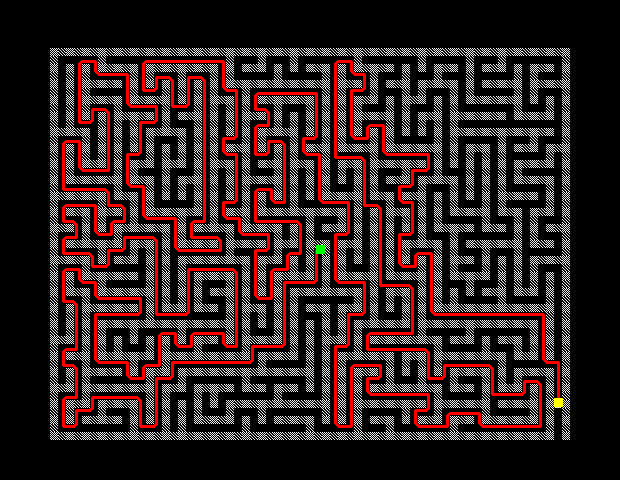
\includegraphics[width=0.82\textwidth]{maze_solution.png}
    \caption{迷宫最短路径结果示意图}
\end{figure}

\subsection*{代码仓库}

\noindent 本题所用 Python 代码以及运行结果已上传至 GitHub 仓库：
\[
\href{https://github.com/zjc20030326/neural-network-models-and-applications.git}
{\texttt{neural-network-models-and-applications}}
\]
\end{document}
